% Created 2026-10-19 lun 11:17
% Intended LaTeX compiler: xelatex
\documentclass{scrartcl}
\usepackage[top=2.5cm, bottom=2.5cm, left=3cm, right=3cm]{geometry}

\usepackage[utf8]{inputenc}
\usepackage[EU1]{fontenc}
\usepackage{graphicx}
\usepackage{grffile}
\usepackage{longtable}
\usepackage{wrapfig}
\usepackage{rotating}
\usepackage[normalem]{ulem}
\usepackage{amsmath}
\usepackage{textcomp}
\usepackage{amssymb}
\usepackage{capt-of}
\usepackage[margin=2cm]{geometry}
\usepackage[dvipsnames]{xcolor}
\usepackage[colorlinks=true, linkcolor=Blue, citecolor=BrickRed, urlcolor=PineGreen]{hyperref}
\usepackage{indentfirst}
\usepackage{minted}
\date{\today}
\title{README - MVP}
\hypersetup{
 pdfauthor={},
 pdftitle={README - MVP},
 pdfkeywords={},
 pdfsubject={},
 pdfcreator={},
 pdflang={English}}
\usepackage{biblatex}

\begin{document}

\maketitle
\tableofcontents

\section{Scope}
\label{sec:org81fe309}
The MVP shows the proof that a joinup-based STI portal will be able to achieve the project aims as defined in the CAPEX proposal and the ATIO design doc.
It will deliver:
\subsection{Sitemap}
\label{sec:org034737e}
\begin{itemize}
\item Welcome: Landing page with access to ATIO and STI collections
\item Collection pages
\begin{itemize}
\item Faceted search
\item Customization of about, logo, banner
\item \texttt{source\_record} (> 100) and \texttt{atio\_innovation} (2-3)
\end{itemize}
\end{itemize}
\subsection{Datamodel}
\label{sec:org3932fd8}
\begin{itemize}
\item \texttt{source\_record}: fully modeled in both RDF and SQL
\item \texttt{atio\_innovation}: fully modeled in both RDF and SQL
\item \texttt{collection}: fully modeled in both RDF and SQL
\item \texttt{claim}: fully modeled in both RDF and SQL
\end{itemize}
\subsection{Curation views}
\label{sec:orgd0fa9e9}
Curators will be able to solve
\begin{itemize}
\item deduplication of \texttt{source\_record}
\item update of a semantic map using skos and projected to the triplestore
\item editing of all 4 types of the current data model in dedicated views
\item QA review of relevant content
\end{itemize}
\subsection{Data access}
\label{sec:org32745c8}
\begin{itemize}
\item \texttt{source\_record} will be readable using REST
\item all data will be accessible using SPARQL
\item \texttt{atio\_innovation} will be writeable using REST
\end{itemize}
\subsection{Out-of-scope}
\label{sec:org765dc2f}
\begin{itemize}
\item ECAs / algorithms transforming \texttt{source\_record} into \texttt{atio\_innovation}
\item Full UX/style copy of current site (e.g. ATIO landing page)
\item Innovation family has to be actually figured out by ATIO
\item Integration with open social will be built later
\item Joinup pruning / new distribution generation will happen later
\end{itemize}
\section{Stakeholders}
\label{sec:org0ce7967}

\begin{center}
\begin{tabular}{ll}
Audience & Expectation\\
\hline
Valeria/Diego & 1. Ontology is implemented as closely as possible, especially when it comes to atio-innovation, innovation families, etc\\
Datalab & Fixed contract of data input format \& APIs (both rest and sparql)\\
Henry & We can actually give everyone (collection) their own landing page, and curation space\\
Alessia & I can do my blueprint work (register innovations in 'Roadmap' following taxonomy defined in blueprint)\\
\end{tabular}
\end{center}
\section{Milestones after MVP}
\label{sec:orge3af0f0}
\subsection{Stable endpoints for REST/SPARQL}
\label{sec:orgd6b00fa}
DEADLINE \textit{<2026-10-29 gio>}
\subsection{Minimal drupal distribution}
\label{sec:org75f992f}
\subsection{Full data input of all STI resources}
\label{sec:orgf89930f}
\begin{itemize}
\item depends on distribution
\end{itemize}
\subsection{User-scoped curation workflow views}
\label{sec:orgd07a97a}
DEADLINE \textit{<2026-10-29 gio>}
\subsection{Tested\&confirmed ATIO data model in system}
\label{sec:org364216c}
DEADLINE \textit{<2026-11-12 gio>}
\subsection{Addtional curation workflows}
\label{sec:org606320f}
\subsection{source record -> atio innovation derivation by AI}
\label{sec:org48f7d11}
DEADLINE \textit{<2026-12-31 gio>}
\subsection{Content display portal -> open social}
\label{sec:orgf488257}
DEADLINE \textit{<2026-11-12 gio>}
\subsection{role mapping open social <-> portal}
\label{sec:org04d66b8}
\section{Documentation of features}
\label{sec:orgf939d2f}
All documentation also lives in the respective modules, a copy for context below
\subsection{REST API and GET access\hfill{}\textsc{datalab}}
\label{sec:org4d0236c}

Joinup uses the \texttt{rest} module (config: /admin/config/services/rest) to define REST endpoints one-by-one. I prefer this over the REST-JSON module, because that one opens REST endpoints to any node in the system. The preferred control to only open access to specific resources makes more sense from a security perspective.
\subsubsection{GET: Collection-scoped content}
\label{sec:org9ca248d}
The relevant GET endpoint is: \texttt{/api/collection-solutions/v1/\{collection\}: GET}. It is defined by the \texttt{sti\_portal\_api} module. It retrieves all content for a given collection. Filters are:
\begin{itemize}
\item \texttt{?moderation=|all|published|unpublished|} : published status. Default: published
\item \texttt{?type=|source\_record|atio\_innovation|} : which content types, comma-separated
\item \texttt{?include=claims} : whether or not to include the claim information. Default: false
\item \texttt{?limit=N} : set a maximum amount to content to retrieve. This copies the pagination on the collection, so a page needs to be speciefied. Default: no limit
\item \texttt{?page=P} : page through results. Default: all pages
\end{itemize}
\subsection{Drupal: \texttt{source\_record} -> \texttt{atio\_innovation} derivation and AI-enrichment}
\label{sec:org95c16bb}
Improving the traceability, quality and modularity of the creation of the \texttt{atio\_innovation} is the core reason for the creation of this MVP. While the STI namespace now handles data input of any strucuture, it results in collections that each present data in their own, unique way. The important step is standardization: The derivation of comparable innovation records requires a centralized format. This is provided by the ATIO team; the only thing changing is the input format of the data they work with to derive this standardized view.
\begin{center}
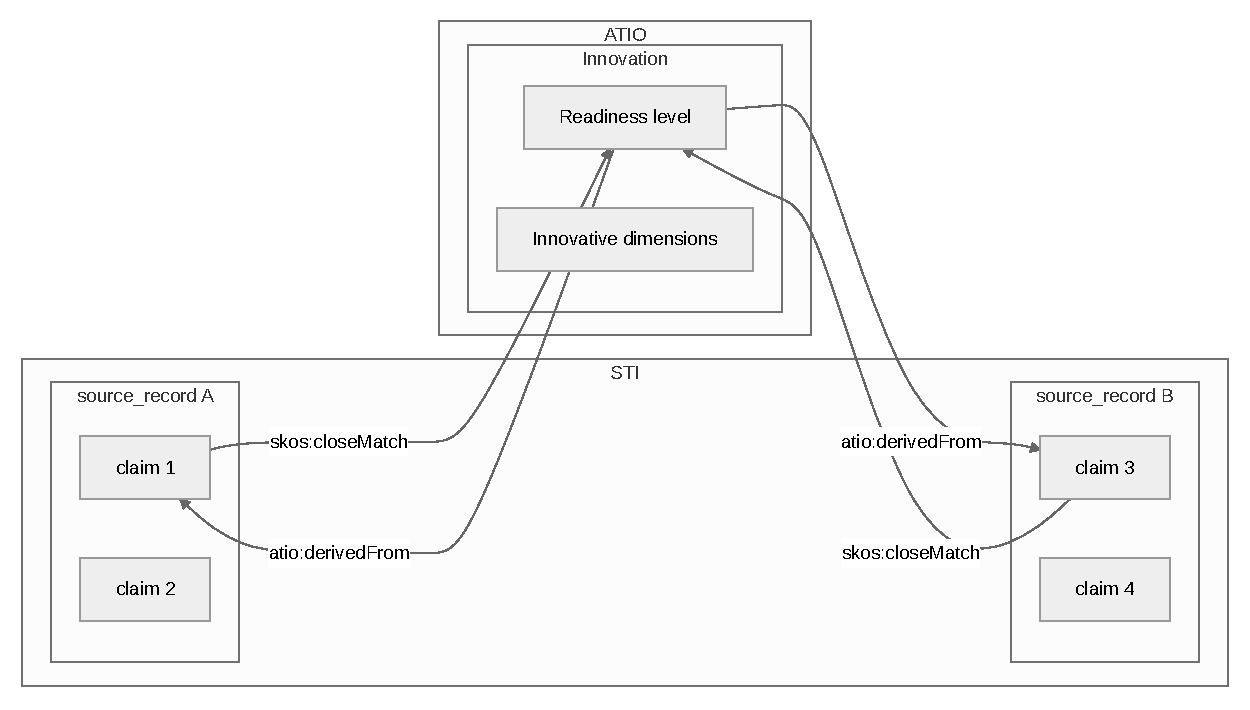
\includegraphics[width=.9\linewidth]{claims-to-atio-flow.pdf}
\label{}
\end{center}
\subsubsection{{\bfseries\sffamily TODO} Next steps\hfill{}\textsc{atio}}
\label{sec:org0f9caf4}
Valeria has created a rather complex claimResolution model. Since historically all \texttt{atio\_innovation} generation has been done by AI and the fact that a single collection easily provides hundreds of thousands of claims, I think claim to \texttt{atio\_innovation} matching will not be done manually. That means we likely will need a more pragmatic claim resolution. Simply by exclusion of \texttt{atio:derivedFrom} statements, decisions of which content is used to fill an \texttt{atio\_innovation} fields are implicitly recorded. In Drupal, this could be modeled as a paragraph \texttt{[field\_derievd\_from}, \texttt{explanation} ] of which only the claim derivation is synced to the triplestore, while the explanation plain text is recorded Drupal-side for potential human revision.
\subsection{Collection / group - scoped permissions handling}
\label{sec:orga671846}
\begin{center}
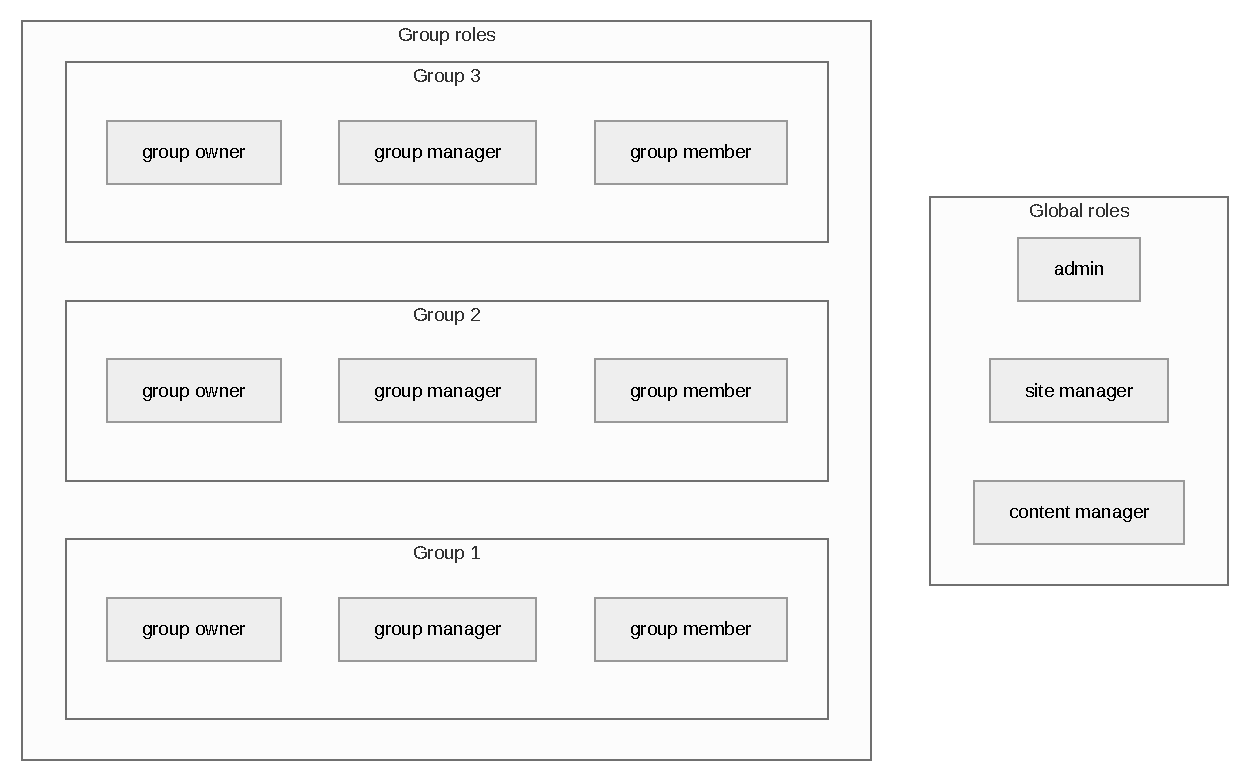
\includegraphics[width=.9\linewidth]{roles.pdf}
\label{}
\end{center}
\section{Documentation of custom modules}
\label{sec:org08132e1}
\subsection{atio}
\label{sec:org1c69261}
This module is a port of the existing core features of the current STI portal implementation. This is mainly a list of content type entities and taxonomy vocabularies. The main difference is a clearer namespace separation to make clear which content belongs to the ATIO work, and which is simply imported to the platform ('sti').
\subsection{\texttt{import\_ird\_json}}
\label{sec:orge0f4833}
\subsection{\texttt{sti\_rdf}}
\label{sec:org16eb778}
\subsubsection{{\bfseries\sffamily TODO} Next steps}
\label{sec:org37308ff}
\begin{itemize}
\item The README.md mentions that this module is responsible for rendering claim facets, but I thought the code in \texttt{import\_ird\_json} is the relevant one for this task?
\end{itemize}
\subsection{\texttt{sti\_graph\_explorer}}
\label{sec:org5db4cb1}
\subsection{\texttt{sti\_dedupe}}
\label{sec:org193394f}
Deduplication is an important task an registered as not fully resolved in the current ATIO design document. It could be done at the \texttt{source\_record} or the \texttt{atio\_innovation} level. This module solves it at the \texttt{source\_record} level. The rationale is that data input from many different sources might likely contain duplicates. Registering this early will allow to map potentially differing claims from different collections about the same \texttt{source\_record} possible. It also makes the derivation of an \texttt{atio\_innovation} easier. Technically this is solved by another field on the claims paragraph: \texttt{duplicate\_of} has claimedAt and claimedBy fields. This also solves the issue of agreement: If collection A claims \texttt{source\_record} A is a duplicate of \texttt{source\_record} B from collection B this statement is recorded. Only if collection B also makes the reverse claim do we have a confirmed agreement.
The module provides an easy interface for data curators to register this duplicate claim.
\subsubsection{{\bfseries\sffamily TODO} Next steps}
\label{sec:orgdad8fef}
\begin{itemize}
\item Role-scoping: Global admin roles should be able to make any claims, collection owners and facilitators can only claim uni-directionally.
\item Role-scoping: The interface should only show potential duplicates to resolve scoped by the current user's role
\item There is already a whole section on claim resolution, but I haven't decided yet how to handle it. It also relies on fields that don't exist yet
\end{itemize}
\subsection{\texttt{sti\_portal\_api}}
\label{sec:org3aa63f9}
This module provides the API endpoint to read a collection's content. It should be the main entrypoint to the system that is being built by the datalab colleagues to get content data. Ideally it is used in conjunction with sparql queries that provide semantic context to the content.
For the data retrieval it is assumed that it is done per-collection and that the user only wishes to filter by publication status, content type and whether or not to add the detailed claims or to only return the content core fields.
\begin{itemize}
\item \texttt{?moderation=|all|published|unpublished|} : published status. Default: published
\item \texttt{?type=|source\_record|atio\_innovation|} : which content types, comma-separated
\item \texttt{?include=claims} : whether or not to include the claim information. Default: false
\item \texttt{?limit=N} : set a maximum amount to content to retrieve. This copies the pagination on the collection, so a page needs to be speciefied. Default: no limit
\item \texttt{?page=P} : page through results. Default: all pages
\end{itemize}
\subsubsection{{\bfseries\sffamily TODO} Next steps}
\label{sec:org0f73d6b}
Access needs to be aligned with the future roles\&permissions model. Ideally, a future version would allow the same group scoping that should exist for the website: Global admin roles can access \& edit any content, but groups also have an owner, facilitator and member scope, where a groups owner and facilitator have read/write access to only their own group's content.
\end{document}
